\documentclass[notes,blackandwhite,mathsans,usenames,dvipsnames]{beamer}

\usepackage{amsmath}
\usepackage{amssymb}
\usepackage{graphicx}
\usepackage{fancybox}
\usepackage{booktabs}
\usepackage{multirow,pxfonts}
\usepackage{cmbright}
\usepackage{xcolor}
\usepackage{color}
\usepackage{enumitem}
\usepackage{animate}
\usepackage{changepage}

\usepackage[T1]{fontenc}
\fontencoding{T1}  
\usepackage[utf8]{inputenc}


\usefonttheme{default}
\setbeamercovered{invisible}
\beamertemplatenavigationsymbolsempty

\makeatletter
\setbeamertemplate{footline}
{
  \leavevmode
  \hbox{
  \begin{beamercolorbox}[wd=0.97\paperwidth,ht=2.25ex,dp=2ex,right]{}
{\color{mcxs2} \insertframenumber{} / \inserttotalframenumber}
  \end{beamercolorbox}}%
}





\definecolor{mcxs1}{HTML}{05386B}
\definecolor{mcxs2}{HTML}{379683}
\definecolor{mcxs3}{HTML}{5CDB95}
\definecolor{mcxs4}{HTML}{8EE4AF}
\definecolor{mcxs5}{HTML}{EDF5E1}
\setbeamercolor{frametitle}{fg=mcxs2}
\AtBeginDocument{\color{mcxs1}}
\setbeamertemplate{itemize item}[triangle]





\begin{document}
%\fontfamily{pag}\selectfont
%\setbeamerfont{title}{family=\fontfamily{pag}\selectfont}
%\setbeamerfont{frametitle}{family=\fontfamily{pag}\selectfont}
%\setbeamerfont{framesubtitle}{family=\fontfamily{pag}\selectfont}






{\setbeamercolor{background canvas}{bg=mcxs2}
\begin{frame}

\vspace{1cm}
\begin{tabular}{rl}
&\textbf{\LARGE\color{mcxs3} Macroeconometrics}\\[8ex]
\textbf{\Large Lecture 14}&\textbf{\Large\color{mcxs5}SVARs: Bayesian estimation II}\\[19ex]
&\textbf{Tomasz Wo\'zniak}\\[1ex]
&{\small\color{mcxs5} Department of Economics}\\
&{\small\color{mcxs5}University of Melbourne}
\end{tabular}

\end{frame}
}






{\setbeamercolor{background canvas}{bg=mcxs2}
\begin{frame}

\vspace{1cm}\textbf{\color{mcxs1}Maximum likelihood estimation}

\bigskip\textbf{\color{purple}Structural VARs with exclusion restrictions}

\smallskip\hspace{0.8cm}\textbf{\color{mcxs1}Useful distribution: normal-generalized-normal}

\bigskip\textbf{\color{mcxs1}Prior and posterior distributions}

\bigskip\textbf{\color{mcxs1}Gibbs sampler}

\bigskip\textbf{\color{mcxs1}Normalization}

\small\vspace{0.8cm} Compulsory reading: \scriptsize

\smallskip{\color{mcxs5}Wo\'zniak (2021) Bayesian Structural VARs: Algorithms and Inference, Lecture notes}


\bigskip Useful readings: \scriptsize

\smallskip{\color{mcxs5}Waggoner \& Zha (2003) A Gibbs sampler for structural vector autoregressions, Journal of Economic Dynamics \& Control}

\smallskip{\color{mcxs5}Waggoner \& Zha (2003) Likelihood preserving normalization in multiple equation models, Journal of Econometrics}

\end{frame}
}






{\setbeamercolor{background canvas}{bg=mcxs2}
\begin{frame}

\bigskip\textbf{\color{mcxs1}Objectives.}
\begin{itemize}[label=$\blacktriangleright$]
\item {\color{mcxs1}To present the most useful frequentists and Bayesian methods}
\item {\color{mcxs1}To introduce an efficient Bayesian estimation algorithm}
\item {\color{mcxs1}To provide tools to work reliably with SVARs }
\end{itemize}

\bigskip\textbf{\color{mcxs4}Learning outcomes.}
\begin{itemize}[label=$\blacktriangleright$]
\item {\color{mcxs4}Implementing concentrated likelihood }
\item {\color{mcxs4}Generating random draws from a normal-generalized-normal distribution}
\item {\color{mcxs4}Applying normalisation to estimation output}
\end{itemize}

\end{frame}
}















{\setbeamercolor{background canvas}{bg=mcxs2}
\begin{frame}

\begin{adjustwidth}{-0.5cm}{0cm}
\vspace{8.3cm}\Large
\textbf{{\color{mcxs1}Maximum likelihood} {\color{mcxs4}estimation}}
\end{adjustwidth}

\end{frame}
}




\begin{frame}{Maximum likelihood estimation: model setup}

\begin{align*}
y_t &= \mu_0 + A_1y_{t-1} + \dots + A_py_{t-p} + Bu_t\\
&=  Ax_{t} + Bu_t\\
u_t|y_{t-1},\dots ,y_{t-p} &\sim iid\mathcal{N}\left(\mathbf{0}_N,I_N\right)
\end{align*}

\bigskip\textbf{Matrix notation.}
\begin{align*}
Y &=  AX + BU\\
U|X &\sim\mathcal{MN}_{N\times T}\left(\mathbf{0}_{N\times T}, I_T, I_N\right)
\end{align*}

\footnotesize
\begin{align*}
\underset{N\times T}{Y} &= \begin{bmatrix} y_1 &\dots& y_T \end{bmatrix} &
\underset{N\times K}{A}&= \begin{bmatrix} \mu_0& A_1 &\dots& A_p \end{bmatrix}\\
\underset{K\times T}{X} &= \begin{bmatrix} x_1 &\dots& x_T \end{bmatrix}&
\underset{K\times 1}{x_t}&= \begin{bmatrix} 1 & y_{t-1}' &\dots& y_{t-p}' \end{bmatrix}'\\
\underset{N\times T}{U} &= \begin{bmatrix} u_1 &\dots& u_T \end{bmatrix}&&
\end{align*}
\end{frame}




\begin{frame}{MLE for SVARs with exclusion restrictions}
\small
\begin{description}
\item[Step 1:] {\color{mcxs2}Obtain the MLE of the RF model} $\left(\widehat{A},\widehat{\Sigma}\right)$
\item[Step 2a:] {\color{mcxs2}If lower-triangular identification is required compute the SF~model MLE by} $\widehat{B}=chol(\widehat\Sigma)$ {\color{mcxs2}and  return} $\left(\widehat{A},\widehat{B}\right)$
\item[Step 2b:] {\color{mcxs2}If other identifying exclusion restrictions are required that are available by the application of} \textbf{Algorithm 1}{\color{mcxs2}, then apply this algorithm to find matrix} $Q${\color{mcxs2}, compute} $\widehat{B}^*=\widehat{B}Q' ${\color{mcxs2}, return:} $\left(\widehat{A},\widehat{B}^*\right)$
\item[Step 2c:] {\color{mcxs2}If non-linear restrictions or restrictions that are not feasible through the application of} \textbf{Algorithm 1} {\color{mcxs2}are required, then use the} \textbf{concentrated maximum likelihood estimation} {\color{mcxs2}method presented below.}
\item[Step 3:] {\color{mcxs2}Apply the invariance property of the MLE to compute} $$\left( \widehat{B}_+, \widehat{B}_0 \right)=\left( \widehat{B}^{-1}\widehat{A}, \widehat{B}^{-1} \right)$$
{\color{mcxs2}and other functions of the parameters such as the IRFs and FEVD}
\item[Step 4:] {\color{mcxs2}Use bootstrap procedure to compute the MLE's standard errors\\ \footnotesize
MacKinnon (2006, ER) and Herwartz, Lange (2020, OREEF)}
\end{description}

\end{frame}







%\begin{frame}{Maximum likelihood estimation}
%
%{\color{mcxs2}Consider SF form parameters} $(A,B)= \left(B_0^{-1}B_+,B_0^{-1}\right)$ {\color{mcxs2}with any exclusion and non-linear restrictions imposed on} $(A,B)$ {\color{mcxs2}such that} $B$ {\color{mcxs2}is non-singular.}
%
%\bigskip\textbf{Log-likelihood function.}\footnotesize
%\begin{align*}
%l(A,B|Y,X) &\propto -T\log\text{det}\left( B\right)  -\frac{1}{2}\text{tr}\left[ (BB')^{-1}(Y-AX)(Y-AX)' \right]\\
%&= -T\log\text{det}\left( B\right)  -\frac{1}{2}\text{tr}\left[ (BB')^{-1}(YY' -2YX'A' + AXX'A' \right]
%\end{align*}
%
%\end{frame}




\begin{frame}{Maximum likelihood estimation}

\bigskip\textbf{Log-likelihood function.}\footnotesize
\begin{align*}
l(A,B|Y,X) &\propto -T\log\text{det}\left( B\right)  -\frac{1}{2}\text{tr}\left[ (BB')^{-1}(Y-AX)(Y-AX)' \right]\\
&= -T\log\text{det}\left( B\right)  -\frac{1}{2}\text{tr}\left[ (BB')^{-1}(YY' -2YX'A' + AXX'A' \right]
\end{align*}


\normalsize
\bigskip\textbf{MLE of $A$.}\footnotesize
\begin{align*}
\frac{\partial l(A,B|Y,X)}{\partial A} &=-\frac{1}{2}\left[ -2(BB')^{-1}YX' + 2(BB')^{-1}AXX' \right]\\
&=(BB')^{-1}YX' -(BB')^{-1}AXX'\\[3ex]
(\widehat{B}\widehat{B}')^{-1}YX' -(\widehat{B}\widehat{B}')^{-1}\widehat{A}XX' =&\; \mathbf{0}_{N\times (1+Np)}\\
YX' -\widehat{A}XX' =&\; \mathbf{0}_{N\times (1+Np)}\\
\widehat{A}XX' =& YX'  \\
\widehat{A} =& YX' (XX')^{-1}
\end{align*}

\end{frame}




\begin{frame}{Maximum likelihood estimation}

\bigskip\textbf{MLE of $B$ using concentrated log-likelihood function.}

\bigskip
\begin{description}
\item[Analytical solution] {\color{mcxs2}for} $\widehat{A}$ {\color{mcxs2}is plugged in the log-likelihood function}
\item[Consistency] {\color{mcxs2}of} $\widehat{A}$ {\color{mcxs2}assures the consistency of} $\widehat{B}$
\item[Numerical optimization] {\color{mcxs2}is used to find} $\widehat{B}$
\end{description}
\small
\begin{align*}
l(B|\widehat{A},\widehat\Sigma,Y,X) &\propto -T\log\text{det}\left( B\right)  -\frac{1}{2}\text{tr}\left[ (BB')^{-1}(Y-\widehat{A}X)(Y-\widehat{A}X)' \right]\\
&= -T\log\text{det}\left( B\right)  -\frac{T}{2}\text{tr}\left[ (BB')^{-1}\frac{\widehat{U}\widehat{U}'}{T} \right]\\
&= -T\log\text{det}\left( B\right)  -\frac{T}{2}\text{tr}\left[ (BB')^{-1}\widehat\Sigma \right]\\[2ex]
\widehat{B} &= \underset{B\in\mathbb{B}}{\arg\max}\text{ } l(B|\widehat{A},\widehat\Sigma,Y,X)
\end{align*}
\normalsize
\begin{description}
\item[Use invariance] {\color{mcxs2}property of the MLE to estimate}
$$ \widehat{B}_0 = \widehat{B}^{-1}\qquad\text{and}\qquad \widehat{B}_+= \widehat{B}^{-1}\widehat{A}$$
\end{description}

\end{frame}



\begin{frame}{Maximum likelihood estimation}

\textbf{A small fiscal policy model.}\small
\begin{align*}
B_0 y_{t} &= b_0 + B_1 y_{t-1} + \dots + B_p y_{t-p} + B u_t\\
u_t|y_{t-1}, \dots, y_{t-p} &\sim iid \mathcal{N}\left( \mathbf{0}_N, \text{diag}\left(\sigma^2\right) \right)
\end{align*}

\normalsize\textbf{Identification.}\small
\begin{align*}
B_0 y_{t} &=  \dots  + B u_t\\
\begin{bmatrix} 1 &0& - \theta_{gdp} \\ 0 &1&-\gamma_{gdp} \\ -\rho_{ttr} &-\rho_{gs}&1\end{bmatrix}\begin{bmatrix}ttr_t \\gs_t \\ rgdp_t\end{bmatrix} &= \dots + \begin{bmatrix} 1 &\theta_{gs}& 0 \\ \gamma_{ttr} &1&0 \\ 0 &0&1\end{bmatrix}\begin{bmatrix}u_t^{(ttr)}\\u_t^{(gs)}\\u_t^{(gdp)} \end{bmatrix}
\end{align*}

\footnotesize
$ttr_t$ {\color{mcxs2}-- total tax revenue,} $gs_t$ {\color{mcxs2}-- government spendings,} $gdp_t$ {\color{mcxs2}-- gross domestic product. All variables are expressed in log, real, per capita terms.}

\bigskip {\color{mcxs2}The system is not identified. See the identification of this system as discussed in Mertens, Ravn (2014, JME)} \emph{A Reconciliation of SVAR and Narrative Estimates of Tax Multipliers} {\color{mcxs2}and the follow up literature.}
\end{frame}







\begin{frame}{Maximum likelihood estimation}

\bigskip{\color{mcxs2}Premultiply the model equation by} $B_0^{-1}$ {\color{mcxs2}to obtain:}\small
\begin{align*}
y_{t} &= \mu_0 + A_1 y_{t-1} + \dots + A_p y_{t-p} + B_0^{-1}B u_t\\
u_t|y_{t-1}, \dots, y_{t-p} &\sim iid \mathcal{N}\left( \mathbf{0}_N, \text{diag}\left(\sigma^2\right) \right)
\end{align*}

\bigskip\normalsize\textbf{RF and SF parameters relationships.}\small
\begin{align*}
A &= B_0^{-1}B_+\\
\Sigma &= B_0^{-1}B \text{diag}\left(\sigma^2\right) B'B_0^{-1\prime}
\end{align*}

\bigskip\normalsize\textbf{Use the MLE.}\small
\begin{align*}
\widehat{A} &= YX' (XX')^{-1}\\
\widehat{U}&=Y-\widehat{A}X\\
\widehat\Sigma &= T^{-1}\widehat{U}\widehat{U}'
\end{align*}


\end{frame}




\begin{frame}{Maximum likelihood estimation}

\bigskip\normalsize\textbf{Concentrated likelihood function.}\small
\begin{align*}
l(B|\widehat{A},\widehat\Sigma,Y,X) &\propto -T\log\text{det}\left( B\right) +T\log\text{det}\left( B_0\right) -\frac{T}{2}\sum_{n=1}^N\log\sigma_n^2\\
&\qquad  -\frac{T}{2}\text{tr}\left[ \left(B_0^{-1}B \text{diag}\left(\sigma^2\right) B'B_0^{-1\prime}\right)^{-1}\widehat\Sigma \right]
\end{align*}

\bigskip\normalsize\textbf{SF parameters MLE.}\small
\begin{align*}
\left(\widehat{B}_0,\widehat{B},\widehat\sigma^2\right) &= \underset{B_0,B,\sigma^2\in\Theta}{\arg\max} l(B_0,B,\sigma^2|\widehat{A},\widehat\Sigma,Y,X)\\
\widehat{B}_+ &= \widehat{B}_0 \widehat{A}
\end{align*}

\bigskip\normalsize\textbf{Useful formulae.}\footnotesize
\begin{align*}
\det(AB) = \det(A)\det(B), \quad \det(A') = \det(A)\\ 
\det\left(A^{-1}\right) = \left(\det(A)\right)^{-1}, \quad \det(\text{diag}(a)) = \prod_{n=1}^N a_n
\end{align*}


\end{frame}








{\setbeamercolor{background canvas}{bg=mcxs2}
\begin{frame}

\begin{adjustwidth}{-0.5cm}{0cm}
\vspace{8.3cm}\Large
\textbf{{\color{mcxs1}Structural VARs with} {\color{mcxs4}exclusion restrictions}}
\end{adjustwidth}

\end{frame}
}




\begin{frame}{Structural VARs with exclusion restrictions}
%\small
\begin{description}
\item[Algorithm 1] {\color{mcxs2}by} Rubio-Ram\'irez, Waggoner, \& Zha (2010) {\color{mcxs2}was based on some initial values} $(\tilde{B}_+,\tilde{B}_0)$

\bigskip\item[In Lecture 13] {\color{mcxs2}we transformed the RF parameters} $(A,\Sigma)$

\bigskip\item[Gibbs sampler] {\color{mcxs2}by} Waggoner \& Zha (2003) {\color{mcxs2}presented today allows reasonable flexibility of imposing zero restrictions for}
	\begin{itemize}[label=\textbullet,leftmargin = *]
	\item {\color{mcxs2}recursive and non-recursive identification patterns}
	
	\smallskip\item {\color{mcxs2}over-identifying restrictions (more than} $N(N-1)/2${\color{mcxs2}) restrictions}
	\end{itemize}
\end{description}

\end{frame}






\begin{frame}{Structural VARs with exclusion restrictions}
%\small
\begin{description}
\item[Gibbs sampler] {\color{mcxs2}by} Waggoner \& Zha (2003) {\color{mcxs2}features:}
\item[A great flexibility] {\color{mcxs2}in the model specification includes:}
	\begin{itemize}[label=\textbullet,leftmargin = *]
	\item {\color{mcxs2}conditional heteroskedasticity}
	\item {\color{mcxs2}time-variation in the parameters}
	\end{itemize}
\item[Facilitates] {\color{mcxs2} Bayesian model comparison and selection}
	
\item[Can be also used] {\color{mcxs2}to sample initial values of parameters} $(\tilde{B}_+,\tilde{B}_0)$ {\color{mcxs2}if the model specification does not allow for sampling} $(A,\Sigma)$ {\color{mcxs2}easily.}

\item[Further extensions] {\color{mcxs2}include SVARs:}
	\begin{itemize}[label=\textbullet,leftmargin = *]
	\item {\color{purple}identified through heteroskedasticity} {\color{mcxs2}and non-normal residuals}
	\item {\color{mcxs2}identified by zero and sign restrictions}
	\item {\color{mcxs2}identified using instrumental variables (Proxy SVARs)}
	\end{itemize}
\end{description}

\end{frame}






\begin{frame}{Structural VARs with exclusion restrictions}

\begin{align*}
B_0y_t &= b_0 + B_1y_{t-1}+ \dots + B_py_{t-p} + u_t\\
&= B_+ x_t + u_t\\[2ex]
{\color{mcxs2}B_+} & \;{\color{mcxs2}= \begin{bmatrix} b_0 & B_1 & \dots & B_p \end{bmatrix}}\\
{\color{mcxs2}x_t} &\;{\color{mcxs2}= \begin{bmatrix} 1 & y_{t-1}' & \dots & y_{t-p}' \end{bmatrix}'}
\end{align*}
%\scriptsize {\color{mcxs2}$B_+ = \begin{bmatrix} b_0 & B_1 & \dots & B_p \end{bmatrix}\qquad x_t' = \begin{bmatrix} 1 & y_{t-1}' & \dots & y_{t-p}' \end{bmatrix}$}

\bigskip\normalsize\textbf{Exclusion restrictions on the rows of} $B_0$.
$$
\underset{\color{mcxs2}(1\times N)}{B_{0[n\cdot]}} = \underset{\color{mcxs2}(1\times r_n)}{b_n} \underset{\color{mcxs2}(r_n\times N)}{V_n} \qquad\text{\color{mcxs2}such that}\qquad
B_0 = \begin{bmatrix} b_1V_1\\ \vdots \\ b_NV_N \end{bmatrix}
$$
\begin{description}
\item[$b_n$] {\color{mcxs2}-- a $1\times r_n$ vector of unrestricted elements of $n$ row of $B_0$}
\item[$V_n$] {\color{mcxs2}-- an $r_n\times N$ {\color{purple}fixed} matrix of ones and zeros}
\end{description}

\bigskip{\color{mcxs2} E.g.:} \small
$
b_n = \begin{bmatrix} b_1 & b_2\end{bmatrix}\quad V_n = \begin{bmatrix} 1&0&0\\0&0&1\end{bmatrix} \quad\rightarrow\quad B_{0[n\cdot]} = \begin{bmatrix} b_1&0 & b_2\end{bmatrix}
$

\end{frame}






\begin{frame}{Structural VARs with exclusion restrictions}

\bigskip\textbf{The $n$th equation.}
\begin{align*}
b_nV_ny_t &= B_n x_t + u_{n.t}\\
u_{n.t} &\sim\mathcal{N}(0,1)\\[1ex]
\downarrow&\\[1ex]
b_nV_nY &= B_n X + U_n\\
U_n &\sim\mathcal{N}\left(\mathbf{0}_T,I_T\right)\\[3ex]
\underset{\color{mcxs2}(N\times T)}{Y}  &= \begin{bmatrix} y_1 & \dots & y_T \end{bmatrix}\\
\underset{\color{mcxs2}(K\times T)}{X}  &= \begin{bmatrix} x_1 & \dots & x_T \end{bmatrix}\\
\underset{\color{mcxs2}(1\times T)}{U_n}  &= \begin{bmatrix} u_{n.1} & \dots & u_{n.T} \end{bmatrix}\\[1ex]
\underset{\color{mcxs2}(1\times K)}{B_n} &= B_{+[n\cdot]}
\end{align*}

\end{frame}



\begin{frame}{Structural VARs with exclusion restrictions}

\textbf{Likelihood function.}\scriptsize
\begin{align*}
L(B_+,B_0|Y,X) &\propto \text{det}\left( B_0^{-1}B_0^{-1\prime} \right)^{-\frac{T}{2}}\exp\left\{ -\frac{1}{2}\sum_{n=1}^N (b_nV_nY - B_n X)(b_nV_nY - B_n X)' \right\}\\
&= |\text{det}\left( B_0 \right)|^{T}\exp\left\{ -\frac{1}{2}\sum_{n=1}^N (b_nV_nY - B_n X)(b_nV_nY - B_n X)' \right\}\\
&= \left|\text{det}\left( \begin{bmatrix} b_1V_1\\ \vdots \\ b_NV_N \end{bmatrix} \right)\right|^{T}\exp\left\{ -\frac{1}{2}\sum_{n=1}^N (b_nV_nY - B_n X)(b_nV_nY - B_n X)' \right\}
\end{align*}

%\bigskip\normalsize\textbf{Useful operations.}\scriptsize
%$$ \text{det}(AB)=\text{det}(A)\text{det}(B)\qquad \text{det}(A')=\text{det}(A) \qquad \text{det}\left(A^{-1}\right)=\text{det}(A)^{-1}$$
\end{frame}






%{\setbeamercolor{background canvas}{bg=purple}
%\begin{frame}
%
%\begin{adjustwidth}{-0.5cm}{0cm}
%\vspace{8.3cm}\Large
%\textbf{{\color{lightgray}Useful distribution:} {\color{white}normal-generalized-normal}}
%\end{adjustwidth}
%
%\end{frame}
%}




\begin{frame}{Useful distribution: {\color{purple}Normal-generalized-normal}}

%\small 
\bigskip
{\color{mcxs2}Let} $1\times K$ {\color{mcxs2}vectors} $B_n$ {\color{mcxs2}and} $1\times r_n$ {\color{mcxs2}vectors} $b_n$ {\color{mcxs2}for} $n=1,\dots,N$ {\color{mcxs2}follow:}
\begin{align*}
p(B_+,B_0)&\sim\mathcal{NGN}\left( \tilde{B}, \Omega, S , \nu  \right)\\
&= \left(\prod_{n=1}^{N}p(B_n|b_n)\right)p(b_1,\dots,b_N)\\[1ex]
p(B_n|b_n) &=\mathcal{N}_K\left(b_nV_n\tilde{B},\Omega \right)\quad{\color{mcxs2}\text{for }n=1,\dots,N}\\
p(b_1, \dots,b_n) &\propto |\text{det}(B_0)|^{\nu-N}\exp\left\{ -\frac{1}{2}\sum_{n=1}^N b_nV_nS^{-1}V_n'b_n'\right\}
\end{align*}
\footnotesize $\tilde{B}$ {\color{mcxs2}-- an} $N\times K$ {\color{mcxs2}matrix;} $\underset{K\times K}{\Omega}$ {\color{mcxs2}and} $\underset{N\times N}{S}$ {\color{mcxs2}-- positive definite matrices;} $\nu\geq N$

\bigskip\normalsize\textbf{Kernel.}\scriptsize
$$
\underbrace{|\text{det}(B_0)|^{\nu-N}\exp\left\{ -\frac{1}{2}\sum_{n=1}^N b_nV_nS^{-1}V_n'b_n'\right\}}_{\text{generalized-normal}}
\underbrace{\exp\left\{ -\frac{1}{2}\sum_{n=1}^N (B_n-b_nV_n\tilde{B})\Omega^{-1}(B_n-b_nV_n\tilde{B})'\right\}}_{\text{conditional normal}}
$$
\end{frame}










\begin{frame}{Structural VARs with exclusion restrictions}

\textbf{Likelihood function as $\mathcal{NGN}$ distribution.}\scriptsize
\begin{align*}
L(B_+,B_0|Y,X) &\propto  |\text{det}\left( B_0 \right)|^{T}\exp\left\{ -\frac{1}{2}\sum_{n=1}^N (b_nV_nY - B_n X)(b_nV_nY - B_n X)' \right\}\\
&= |\text{det}\left( B_0 \right)|^{T}\exp\left\{ -\frac{1}{2}\sum_{n=1}^N (b_nV_nYY'V_n'b_n' -2 b_nV_nYX'B_n' + B_nXX'B_n') \right\}
\end{align*}
\normalsize {\color{mcxs2}Expand the expression from the parentheses:}\tiny
\begin{align*}
b_n&V_nYY'V_n'b_n' -2 b_nV_nYX'B_n' + B_nXX'B_n' =\\
&= b_nV_nYY'V_n'b_n' + B_nXX'B_n' -2 b_nV_nYX'{\color{mcxs2}(XX')^{-1}(XX')}B_n' \pm {\color{mcxs2}b_nV_nYX'(XX')^{-1}(XX')(XX')^{-1}XY'V_n'b_n'}\\
&\qquad{\color{mcxs2}\text{Let } \widehat{A}=YX'(XX')^{-1}}\\
&= b_nV_n\left[YY' - YX'(XX')^{-1}XY'  \right]V_n'b_n' + \left(B_n - b_nV_n\widehat{A}\right)(XX')\left(B_n - b_nV_n\widehat{A}\right)'
\end{align*}
\normalsize {\color{mcxs2}Likelihood function can be presented as:}\small
\begin{align*}
L(B_+,B_0|Y,X) &\sim\mathcal{NGN}\left( \widehat{A},\; (XX')^{-1}, \;(YY' - YX'(XX')^{-1}XY')^{-1} ,\; T+N  \right)
\end{align*}

\end{frame}





{\setbeamercolor{background canvas}{bg=mcxs2}
\begin{frame}

\begin{adjustwidth}{-0.5cm}{0cm}
\vspace{8.3cm}\Large
\textbf{{\color{mcxs1}Prior and posterior} {\color{mcxs4}distributions}}
\end{adjustwidth}

\end{frame}
}




\begin{frame}{Natural-conjugate prior distribution}
\small
{\color{mcxs2}The} $\mathcal{NGN}$ {\color{mcxs2}distribution can be used as a natural-conjugate prior:}
\begin{align*}
p(B_+,B_0)&\sim\mathcal{NGN}\left( \underline{B}, \underline{\Omega}, \underline{S} , \underline{\nu}  \right)\\[2ex]
p(B_+,B_0)&= \left(\prod_{n=1}^{N}p(B_n|b_n)\right)p(b_1,\dots,b_N)\\[1ex]
p(B_n|b_n)&\sim\mathcal{N}_K\left( b_nV_n\underline{B}, \underline{\Omega} \right)\\
p(b_1,\dots,b_N)&\propto |\text{det}(B_0)|^{\underline{\nu}-N}\exp\left\{ -\frac{1}{2}\sum_{n=1}^N b_nV_n\underline{S}^{-1}V_n'b_n'\right\}
\end{align*}

\bigskip\textbf{Kernel.}\scriptsize
$$
|\text{det}(B_0)|^{\underline{\nu}-N}\exp\left\{ -\frac{1}{2}\sum_{n=1}^N b_nV_n\underline{S}^{-1}V_n'b_n'\right\}
\exp\left\{ -\frac{1}{2}\sum_{n=1}^N (B_n-b_nV_n\underline{B})\underline{\Omega}^{-1}(B_n-b_nV_n\underline{B})'\right\}
$$
\end{frame}





\begin{frame}{Posterior distribution}
\small
\begin{align*}
p(B_+&,B_0|Y,X)\propto L(B_+,B_0|Y,X)p(B_+,B_0)\\[2ex]
&= |\text{det}\left( B_0 \right)|^{T}\exp\left\{ -\frac{1}{2}\sum_{n=1}^N (b_nV_nY - B_n X)(b_nV_nY - B_n X)' \right\}\\
&\qquad\times |\text{det}(B_0)|^{\underline{\nu}-N} \exp\left\{ -\frac{1}{2}\sum_{n=1}^N b_nV_n\underline{S}^{-1}V_n'b_n'\right\}\\
&\qquad\times \exp\left\{ -\frac{1}{2}\sum_{n=1}^N (B_n-b_nV_n\underline{B})\underline{\Omega}^{-1}(B_n-b_nV_n\underline{B})'\right\}\\[2ex]
&= |\text{det}\left( B_0 \right)|^{T+\underline{\nu}-N}\\
&\quad\times\exp\left\{ -\frac{1}{2}\sum_{n=1}^N \left(
b_nV_nYY'V_n'b_n' -2 b_nV_nYX'B_n' + B_nXX'B_n' \right.\right.\\
&\quad \left.\left.+ b_nV_n\underline{S}^{-1}V_n'b_n' + 
B_n \underline{\Omega}^{-1} B_n' -2b_nV_n\underline{B}\underline{\Omega}^{-1}B_n' + 
b_nV_n\underline{B}\underline{\Omega}^{-1}\underline{B}'V_n'b_n'
\right) \right\}
\end{align*}

\end{frame}




\begin{frame}{Posterior distribution}
\small
Expression from the parentheses:\scriptsize
\begin{adjustwidth}{-0.7cm}{0cm}
\begin{align*}
b_nV_nY&Y'V_n'b_n' -2 b_nV_nYX'B_n' + B_nXX'B_n' 
+ b_nV_n\underline{S}^{-1}V_nb_n'\\
 &\qquad\qquad\qquad\qquad+ B_n \underline{\Omega}^{-1} B_n' -2b_nV_n\underline{B}\underline{\Omega}^{-1}B_n' + b_nV_n\underline{B}\underline{\Omega}^{-1}\underline{B}'V_n'b_n' \\
&= B_n{\color{mcxs2}\left[XX'  + \underline{\Omega}^{-1} \right]} B_n'
-2 b_nV_n\left[YX' +\underline{B}\underline{\Omega}^{-1}\right]B_n'
+ b_nV_n\left[ YY' + \underline{S}^{-1} + \underline{B}\underline{\Omega}^{-1}\underline{B}'\right]V_n'b_n'\\
&= B_n{\color{mcxs2}\overline{\Omega}^{-1}} B_n'
-2 b_nV_n\left[YX' +\underline{B}\underline{\Omega}^{-1}\right]{\color{mcxs2}\overline{\Omega}}{\color{mcxs2}\overline{\Omega}^{-1}}B_n'
+ b_nV_n\left[ YY' + \underline{S}^{-1} + \underline{B}\underline{\Omega}^{-1}\underline{B}'\right]V_n'b_n'\\
&= B_n\overline{\Omega}^{-1} B_n'
-2 b_nV_n{\color{purple}\left[YX' +\underline{B}\underline{\Omega}^{-1}\right]\overline{\Omega}}\overline{\Omega}^{-1}B_n'
+ b_nV_n\left[ YY' + \underline{S}^{-1} + \underline{B}\underline{\Omega}^{-1}\underline{B}'\right]V_n'b_n'\\
&= B_n\overline{\Omega}^{-1} B_n'
-2 b_nV_n{\color{purple}\overline{B}}\overline{\Omega}^{-1}B_n' \pm{\color{blue}b_nV_n\overline{B}\overline{\Omega}^{-1}\overline{B}'V_n'b_n'}
+ b_nV_n\left[ YY' + \underline{S}^{-1} + \underline{B}\underline{\Omega}^{-1}\underline{B}'\right]V_n'b_n'\\
&= \left( B_n - b_nV_n\overline{B} \right)\overline{\Omega}^{-1}\left( B_n - b_nV_n\overline{B} \right)'
+ b_nV_n{\color{red}\left[ YY' + \underline{S}^{-1} + \underline{B}\underline{\Omega}^{-1}\underline{B}' - \overline{B}\overline{\Omega}^{-1}\overline{B}' \right]}V_n'b_n'\\
&= \left( B_n - b_nV_n\overline{B} \right)\overline{\Omega}^{-1}\left( B_n - b_nV_n\overline{B} \right)'
+ b_nV_n{\color{red}\overline{S}^{-1}}V_n'b_n'\\
\end{align*}
\end{adjustwidth}

\end{frame}




\begin{frame}{Posterior distribution}

\begin{align*}
p(B_+,B_0|Y,X)&\sim\mathcal{NGN}\left( \overline{B}, \overline{\Omega}, \overline{S} , \overline{\nu}  \right)\\[2ex]
\overline{\Omega} &= \left[XX'  + \underline{\Omega}^{-1} \right]^{-1} \\
\overline{B} &= \left[YX' +\underline{B}\underline{\Omega}^{-1}\right]\overline{\Omega} \\
\overline{S} &= \left[ YY' + \underline{S}^{-1} + \underline{B}\underline{\Omega}^{-1}\underline{B}' - \overline{B}\overline{\Omega}^{-1}\overline{B}' \right]^{-1}\\
\overline{\nu} &= T + \underline{\nu}\\[2ex]
&V_1, \dots, V_N
%p(B_+,B_0)&= p(B_n|b_n)p(B_0)\\
%p(B_n|b_n)&\sim\mathcal{N}_K\left( b_nV_n\overline{B}, \overline{\Omega} \right)\\
%p(B_0)&\propto |\text{det}(B_0)|^{\overline{\nu}-N}\exp\left\{ -\frac{1}{2}\sum_{n=1}^N b_nV_n\overline{S}^{-1}V_n'b_n'\right\}
\end{align*}
\end{frame}







{\setbeamercolor{background canvas}{bg=mcxs2}
\begin{frame}

\begin{adjustwidth}{-0.5cm}{0cm}
\vspace{8.3cm}\large
\textbf{{\color{mcxs1}Gibbs sampler} {\color{mcxs4}for normal-generalized-normal distribution}}
\end{adjustwidth}

\end{frame}
}





\begin{frame}{Gibbs sampler}

\textbf{Posterior distribution.}
\begin{align*}
p(B_+,B_0|Y,X)&\sim\mathcal{NGN}\left( \overline{B}, \overline{\Omega}, \overline{S} , \overline{\nu}  \right)\\[2ex]
&= p(B_0|Y,X)\prod_{n=1}^{N}p(B_n|Y,X,b_n)\\
p(B_0|Y,X)&\propto |\text{det}(B_0)|^{\overline{\nu}-N}\exp\left\{ -\frac{1}{2}\sum_{n=1}^N b_nV_n\overline{S}^{-1}V_n'b_n'\right\}\\
p(B_n|Y,X,b_n)&\sim\mathcal{N}_K\left( b_nV_n\overline{B}, \overline{\Omega} \right)
\end{align*}

\begin{description}
\item[Sampler] {\color{mcxs2}for} $p(B_0|Y,X)$ {\color{mcxs2}proceeds row by row and draws from full conditional posterior distributions:}
$$p\left(b_n|Y,X,b_1,\dots,b_{n-1},b_{n+1},\dots,b_N\right)$$
\item[Sampling] {\color{mcxs2}from a multivariate normal} $p(B_n|Y,X,b_n)$ {\color{mcxs2}is simple}
\end{description}


\end{frame}




\begin{frame}{Gibbs sampler}

{\color{mcxs2}Sampling from the} $\mathcal{NGN}$ {\color{mcxs2}distribution is performed in} {\color{purple}two steps:}

\bigskip
\begin{description}
\item[Gibbs sampler for] $B_0$ \\ {\color{mcxs2}Sample} $S$ {\color{mcxs2}draws from}
$p\left(b_n^{(s)}|Y,X,b_1^{(s)},\dots,b_{n-1}^{(s)},b_{n+1}^{(s-1)},\dots,b_N^{(s-1)}\right)$
{\color{mcxs2}obtaining posterior sample} $\left\{ b_1^{(s)}, \dots, b_N^{(s)} \right\}_{s=1}^S$

\bigskip\item[\color{purple}Normalize] {\color{mcxs2}the draws} $\left\{ b_1^{(s)}, \dots, b_N^{(s)} \right\}_{s=1}^S$

\bigskip\item[Direct sampling for] $B_+$ \\
{\color{mcxs2}For each draw of} $b_n^{(s)}$ {\color{mcxs2}draw} $B_n$ {\color{mcxs2}from} $p(B_n|Y,X,b_n)$\\ {\color{mcxs2}for} $n=1,\dots,N$ {\color{mcxs2}and} $s=1,\dots,S$

\bigskip\item[Return] {\color{mcxs2}the sample drawn from the $\mathcal{NGN}$ posterior distribution}
$$ \left\{ B_+^{(s)}, B_0^{(s)} \right\}_{s=1}^{S} $$
\end{description}
\end{frame}



\begin{frame}{Gibbs sampler}
\footnotesize
\bigskip\textbf{Gibbs sampler for $b_n^{(s)}\sim p\left(b_n|Y,X,b_1^{(s)},\dots,b_{n-1}^{(s)},b_{n+1}^{(s-1)},\dots,b_N^{(s-1)}\right)$}
\begin{description}
\item[Compute] the following values:
\begin{align*}
U_n &= chol\left(\overline{\nu} \left(V_n\overline{S}^{-1}V_n'\right)^{-1}\right) {\color{mcxs2}\text{ -- } \text{ an } r_n\times r_n\text{ upper-triangular matrix}}\\
w &= \left[B_{0[-n.\cdot]}^{(s)}\right]_{\bot} {\color{mcxs2}\text{-- where } w \text{ is a }1\times N \text{ matrix}} \\
w_1 &= wV_n'U_n' \cdot \left( wV_n'U_n' U_n V_nw' \right)^{-\frac{1}{2}} {\color{mcxs2}\text{-- where } w_1 \text{ is a } 1\times r_n \text{ vector}}\\
W_n &= \begin{bmatrix}w_1' & w_{1\bot}'\end{bmatrix}' {\color{mcxs2}\text{-- where } W_n \text{ is a } r_n\times r_n \text{ matrix}}
\end{align*}

\item[Draw] the elements of a $1\times r_n$ vector $\alpha_n$:
	\begin{description}
	\item[Draw] the first element of $\alpha_n$ by: 
		\begin{description}
		\item[drawing] $u\sim\mathcal{N}\left( \mathbf{0}_{\nu+1}, \overline{\nu}^{-1}I_{\nu+1} \right)$, and
		\item[setting] $\alpha_{n[\cdot.1]}= \left\{ \begin{array}{ll} \sqrt{u'u} & \text{with probability } 0.5 \\ -\sqrt{u'u} & \text{with probability } 0.5 \end{array} \right.$
		\end{description}
		\item[Draw] the remaining $r_n-1$ elements of $\alpha_n$ from $\mathcal{N}\left( \mathbf{0}_{r_n-1}, \overline{\nu}^{-1}I_{r_n-1} \right)$.
	\end{description}
\item[Compute] the draw from the full conditional posterior distribution of $b_n$ by:
$$ b_n^{(s)} = \alpha_n W_n U_n$$
\end{description}
\end{frame}



\begin{frame}{Gibbs sampler}

{\color{mcxs2}In the description of the Gibbs sampler in the previous slide:}
\begin{description}
\item[$X_{\bot}$] {\color{mcxs2}-- is an orthogonal complement matrix of} $X$ 
\item[$B_{0[-n.\cdot]}^{(s)}$] {\color{mcxs2}-- denotes matrix} $B_{0}^{(s)}$ {\color{mcxs2}without its $n$th row:}
\end{description}

\small
$$ B_{0[-n.\cdot]}^{(s)} = \begin{bmatrix} b_1^{(s)}V_1\\ \vdots \\ b_{n-1}^{(s)}V_{n-1}\\b_{n+1}^{(s-1)}V_{n+1}\\ \vdots \\ b_N^{(s-1)}V_N \end{bmatrix}
$$

\end{frame}





{\setbeamercolor{background canvas}{bg=mcxs2}
\begin{frame}

\begin{adjustwidth}{-0.5cm}{0cm}
\vspace{8.3cm}\Large
\textbf{{\color{lightgray}} {\color{mcxs1}Normalization}}
\end{adjustwidth}

\end{frame}
}


%\begin{frame}
%
%\centering
%\vspace{1cm}\Large\textbf{\color{purple}Normalization} \textbf{\color{mcxs2} }
%
%\end{frame}



\begin{frame}{Normalization}

{\color{mcxs2}The output of the Gibbs sampler perfectly reproduces {\color{purple}the symmetry of the posterior distribution} of matrices} $B_0$ {\color{mcxs2}and} $B_+$ {\color{purple}around zero} {\color{mcxs2}being the effect of local identification. }

\bigskip{\color{mcxs2}The likelihood function and the posterior distribution have} $2^N$ {\color{purple}equal modes} {\color{mcxs2}as a consequence of local identification}

\bigskip{\color{mcxs2}Such an output represents the global shape of the posterior distribution (that is inherited from the likelihood function) and provides the full statistical characterization of these parameters.}

\bigskip{\color{mcxs2}It {\color{purple}cannot be used to compute rotation-dependent characteristics} of the values of interest such as the estimates of the parameters of the model or the impulse response functions. }

\bigskip{\color{mcxs2}The means of these values computed from the unnormalized output will all {\color{purple}be equal to zero}.}

\end{frame}


\begin{frame}{Normalization}

Waggoner \& Zha (2003, JOE) {\color{mcxs2}provide the optimal normalizing rule that preserves the shape of the likelihood function. }

\bigskip{\color{mcxs2}Let} $\widehat{B}_0$ {\color{mcxs2}be one of the} $2^N$ {\color{mcxs2}modes of the posterior distribution with normalized signs of the shocks, that is, with the chosen sign of the rows}

\bigskip{\color{purple}Normalization} {\color{mcxs2}of the posterior sampler output is performed with respect to} $\widehat{B}_0$ {\color{mcxs2}so that its only mode is equal to} $\widehat{B}_0$


\end{frame}



\begin{frame}{Normalization}

{\color{mcxs2}Define a set of} $N\times N$ {\color{mcxs2}diagonal normalizing matrices} $D_i$ {\color{mcxs2}for} $i = 1,\dots , 2^N$

\bigskip{\color{mcxs2}The diagonal elements of} $D_i$ {\color{mcxs2}are equal to} 1 {\color{mcxs2}or} -1 {\color{mcxs2}in all of the possible combinations across} $i$. $D_i$ {\color{mcxs2}are orthogonal matrices.}

\bigskip{\color{mcxs2}These} $2^N$ {\color{mcxs2}matrices} $D_i$ {\color{mcxs2}exhaustively represent all of the possible combinations of ones and minus ones on the} $N$ {\color{mcxs2}elements of the main diagonal}

\end{frame}


\begin{frame}{Normalization}

{\color{mcxs2}The algorithm for normalization utilizes a {\color{purple}distance measure}:}
$$
d\left[ X | \widehat\Sigma \right] = \sum_{n=1}^{N}X_{[n.\cdot]} \widehat\Sigma^{-1} X_{[n.\cdot]}'
$$
\begin{description}
\item[$X$] {\color{mcxs2}-- an} $N\times N$ {\color{mcxs2}matrix}
\item[$X_{[n.\cdot]}$] {\color{mcxs2}-- the} $n${\color{mcxs2}th row of} $X$
\item[$\widehat\Sigma$] {\color{mcxs2}-- an} $N\times N$ {\color{mcxs2}positive definite matrix}
\end{description}

\end{frame}




\begin{frame}{Normalization}

{\color{mcxs2}To normalize the} $s${\color{mcxs2}th draw from the posterior distribution,} $B_0^{(s)}$:
\begin{description}
\item[Compute the distance]  {\color{mcxs2}between} $D_iB_0^{(s)}$ {\color{mcxs2}and} $\widehat{B}_0$:
$$
d\left[ \left( D_i B_0^{(s)} \right)^{-1\prime} - \widehat{B}_0^{-1\prime} \Big| \left( \widehat{B}_0' \widehat{B}_0 \right)^{-1} \right]
$$
{\color{mcxs2}for } $i=1,\dots,2^N$

\bigskip\item[Return] {\color{mcxs2}the normalized draw given by} 
$$D_{i*}B_0^{(s)}$$ 
{\color{mcxs2}where} $i*$ {\color{mcxs2}is the value of} $i$ {\color{mcxs2}that {\color{purple}minimizes the distance} above}

\bigskip\item[Normalize]  $B_0^{(s)}$ {\color{mcxs2}before sampling} $B_+^{(s)}$ {\color{mcxs2}dependent on} $B_0^{(s)}$
\end{description}

\end{frame}



\begin{frame}{Normalization}

\bigskip\textbf{An illustration}
\small
\begin{equation*}
\begin{bmatrix}a_{11}&0&0\\ 0& a_{22}&a_{23}\\a_{31}& a_{32}&a_{33} \end{bmatrix}\begin{bmatrix} gdp_t \\ FF_t \\ pcom_t \end{bmatrix} = \begin{bmatrix} A_{11}& A_{12}& A_{13}\\  A_{21}& A_{22}& A_{23}\\ A_{31}& A_{32}& A_{33} \end{bmatrix}\begin{bmatrix} gdp_{t-1} \\ FF_{t-1} \\ pcom_{t-1} \end{bmatrix} + \begin{bmatrix}  u_{1.t}\\ u_{3.t}\\ u_{3.t}\end{bmatrix}
\end{equation*}

\bigskip\normalsize {\color{mcxs2}Restrictions are imposed using} \small
$$V_1 = \begin{bmatrix}  1&0&0 \end{bmatrix} \qquad V_2 = \begin{bmatrix}  0&1&0 \\ 0&0&1 \end{bmatrix}, \qquad V_3 = \begin{bmatrix}  1&0&0 \\ 0&1&0 \\ 0&0&1 \end{bmatrix}$$

\begin{center}
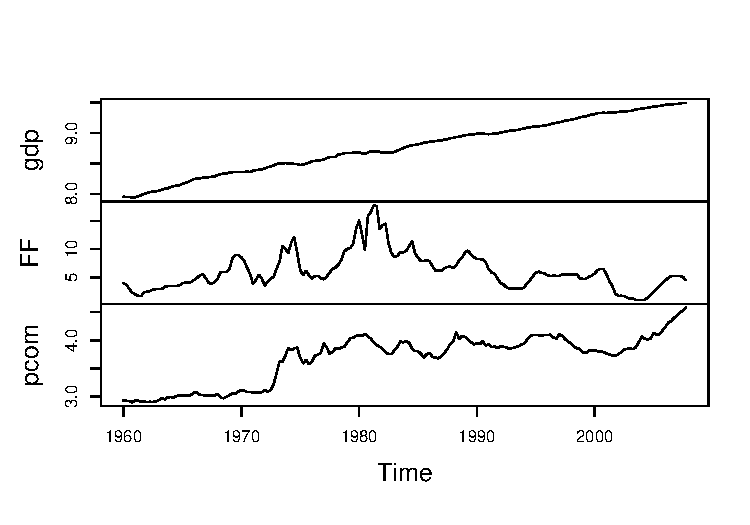
\includegraphics[scale=0.5, trim=0cm 1cm 0cm 1cm]{./Estimation/data.pdf}
\end{center}


\end{frame}


\begin{frame}{Normalization}

\begin{tabular}{cc}
\toprule
non-normalized  & normalized \\
\midrule
\multicolumn{2}{c}{posterior means}\\
$\begin{bmatrix}
-0.001& 0&  0\\
0& 0.001& -0.001\\
0.023& 0.002& -0.058
\end{bmatrix}$
&
$ \begin{bmatrix}
0.081&  0&  0\\
0&  0.231& -0.379\\
-0.994& -0.059&  2.462
\end{bmatrix}$\\[5ex]
%\midrule
\multicolumn{2}{c}{densities: posterior vs. prior: $(a_{22},a_{23})$}\\
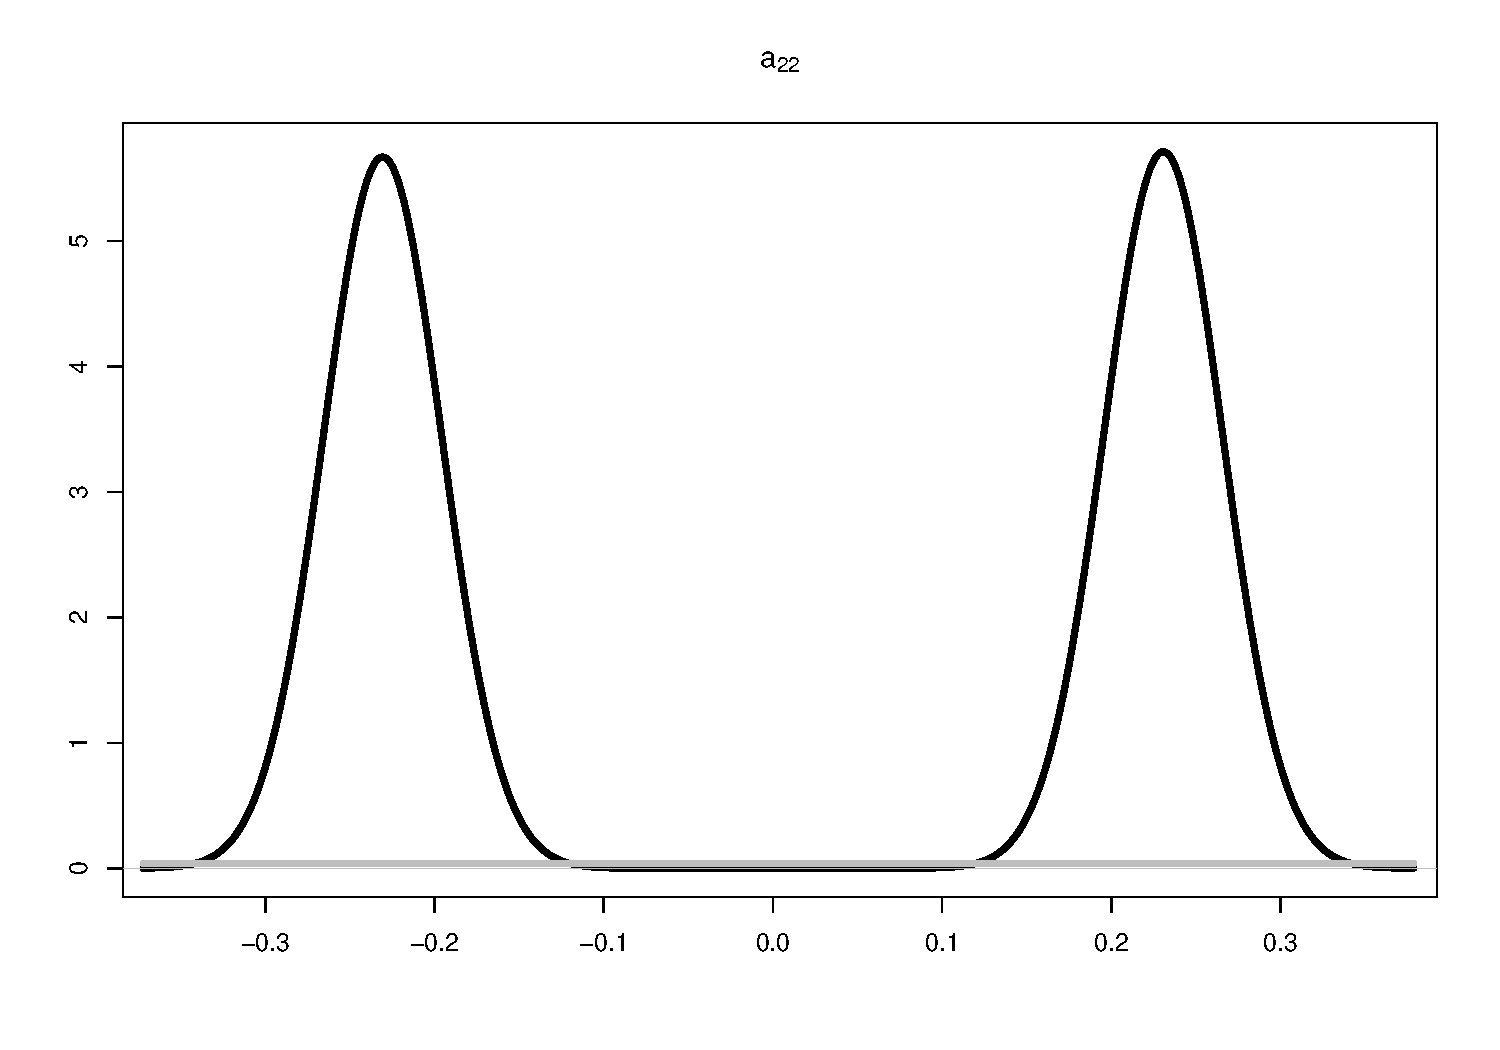
\includegraphics[scale=0.15, trim=0cm 1cm 0cm 1cm]{./Estimation/norm-density-22.pdf}&
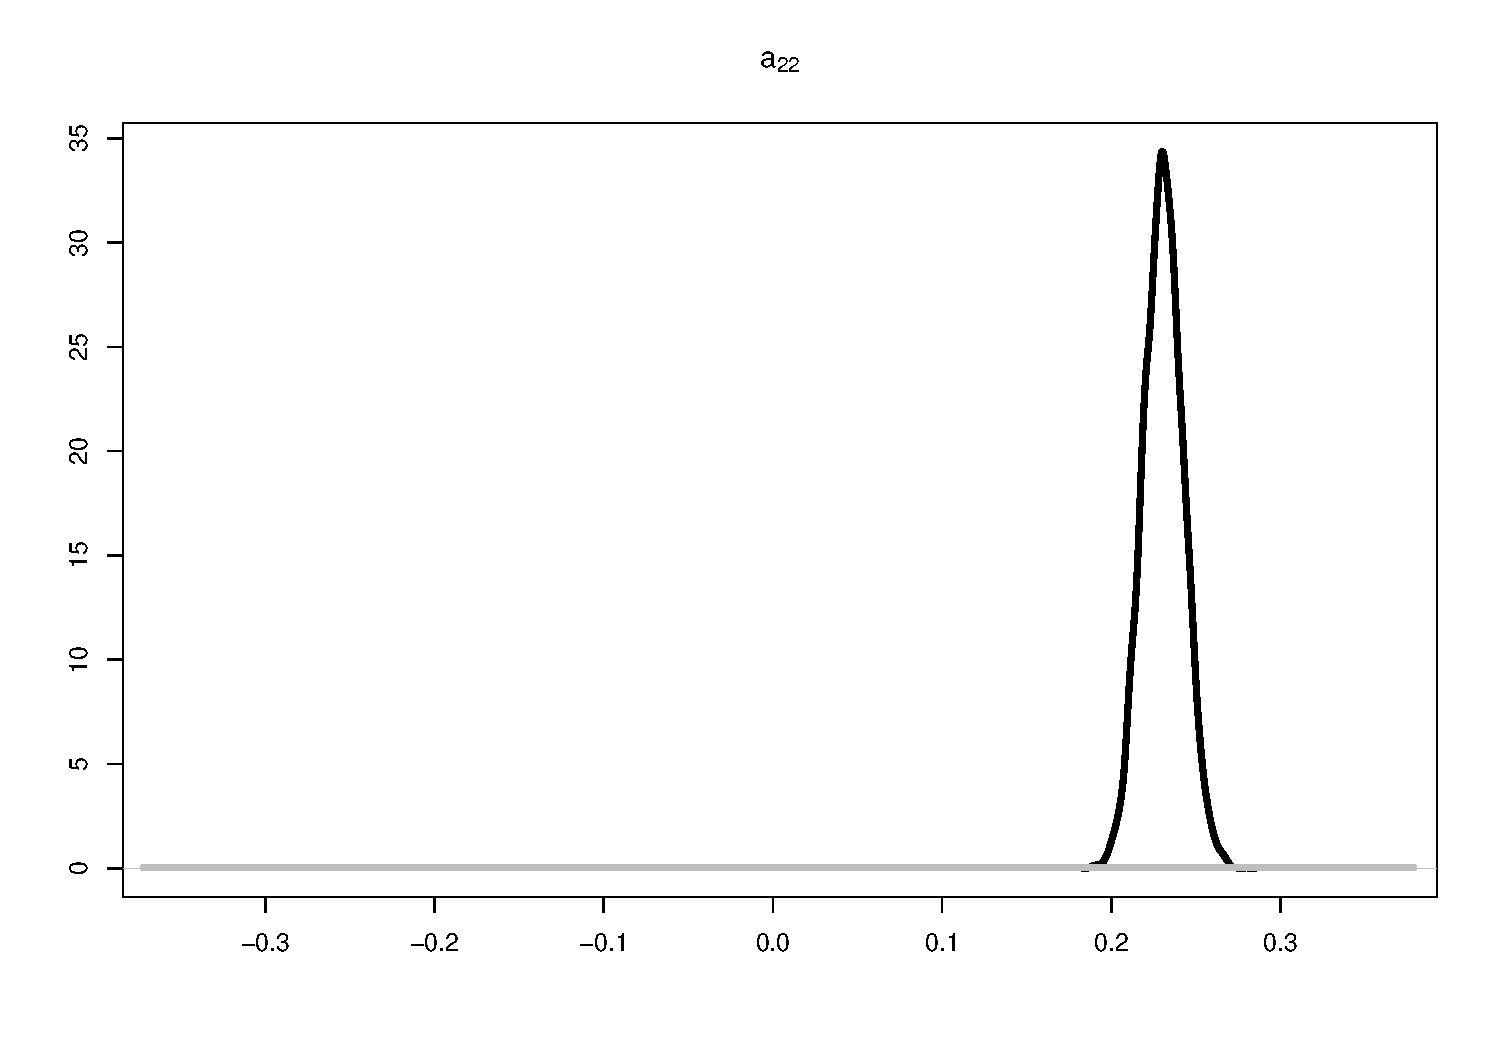
\includegraphics[scale=0.15, trim=0cm 1cm 0cm 1cm]{./Estimation/norm-density-22-n.pdf}\\

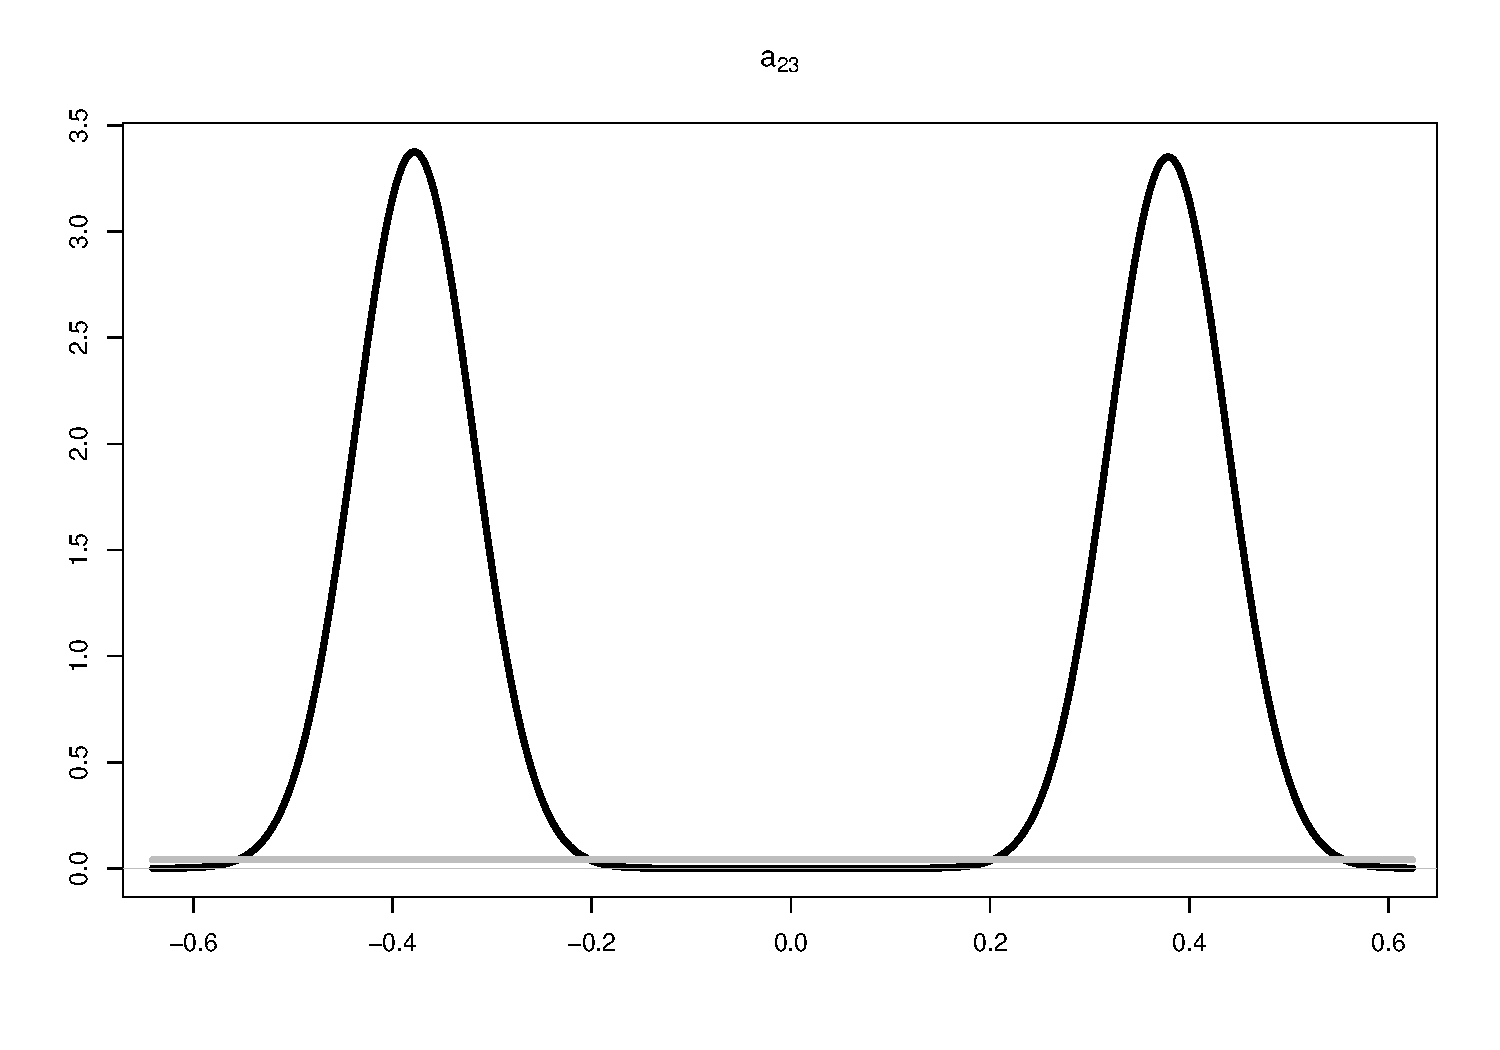
\includegraphics[scale=0.15, trim=0cm 1cm 0cm 1cm]{./Estimation/norm-density-23.pdf}&
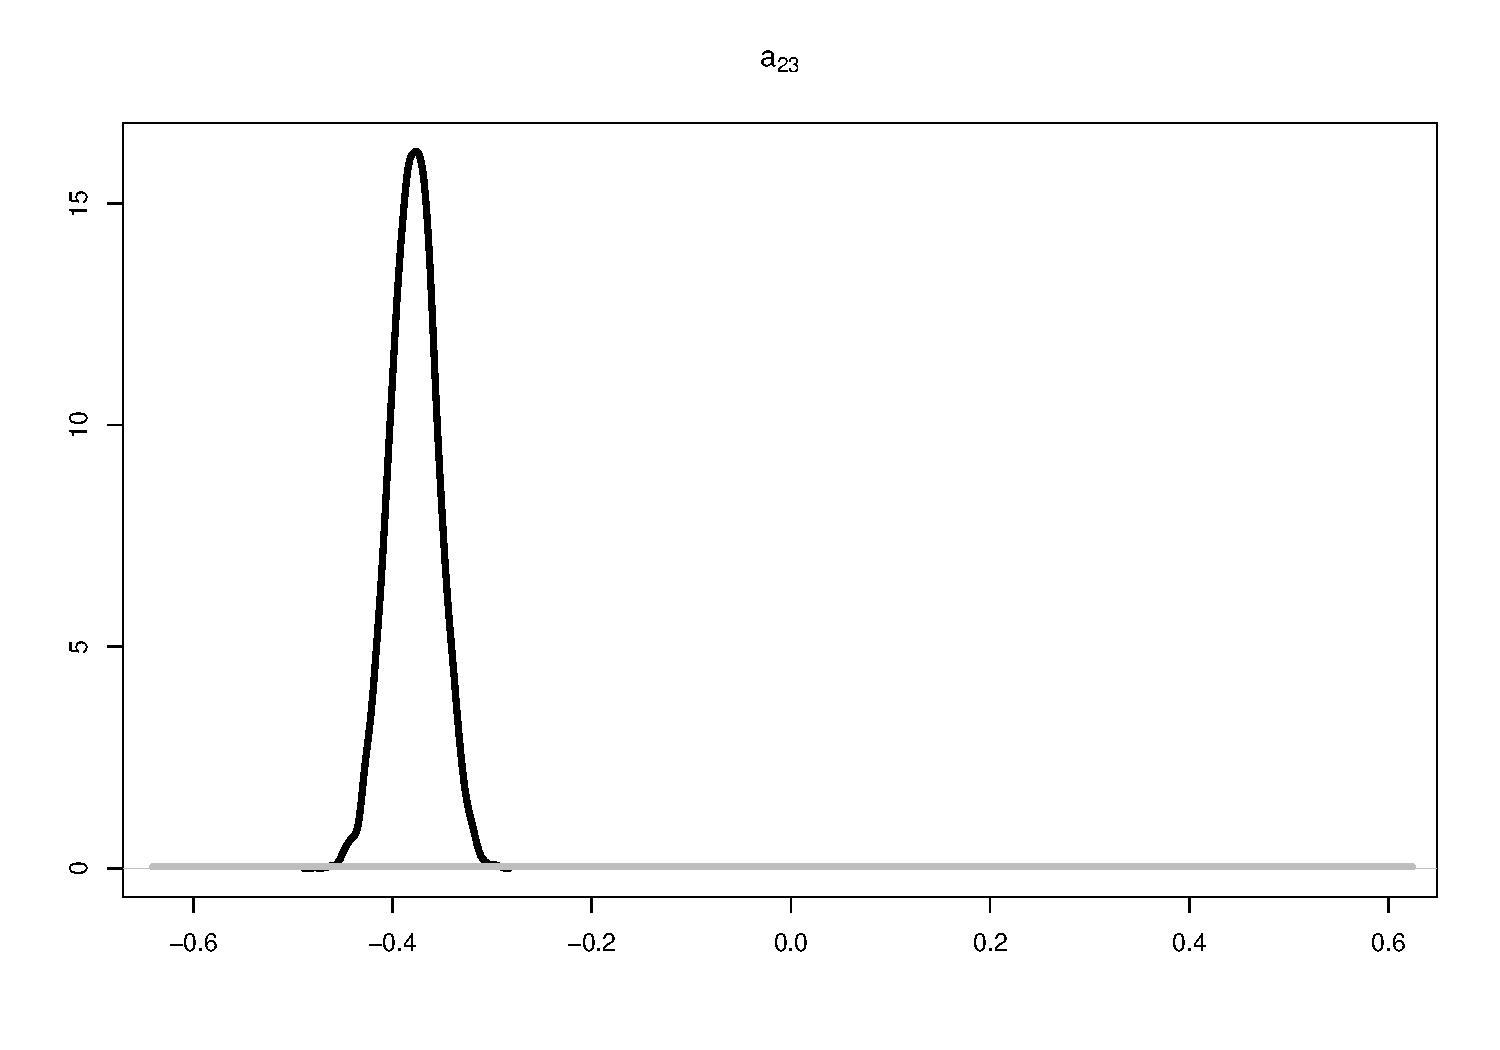
\includegraphics[scale=0.15, trim=0cm 1cm 0cm 1cm]{./Estimation/norm-density-23-n.pdf}\\
%\bottomrule
\end{tabular}

\end{frame}




\begin{frame}{Normalization}

\begin{tabular}{cc}
\toprule
non-normalized  & normalized \\
\midrule
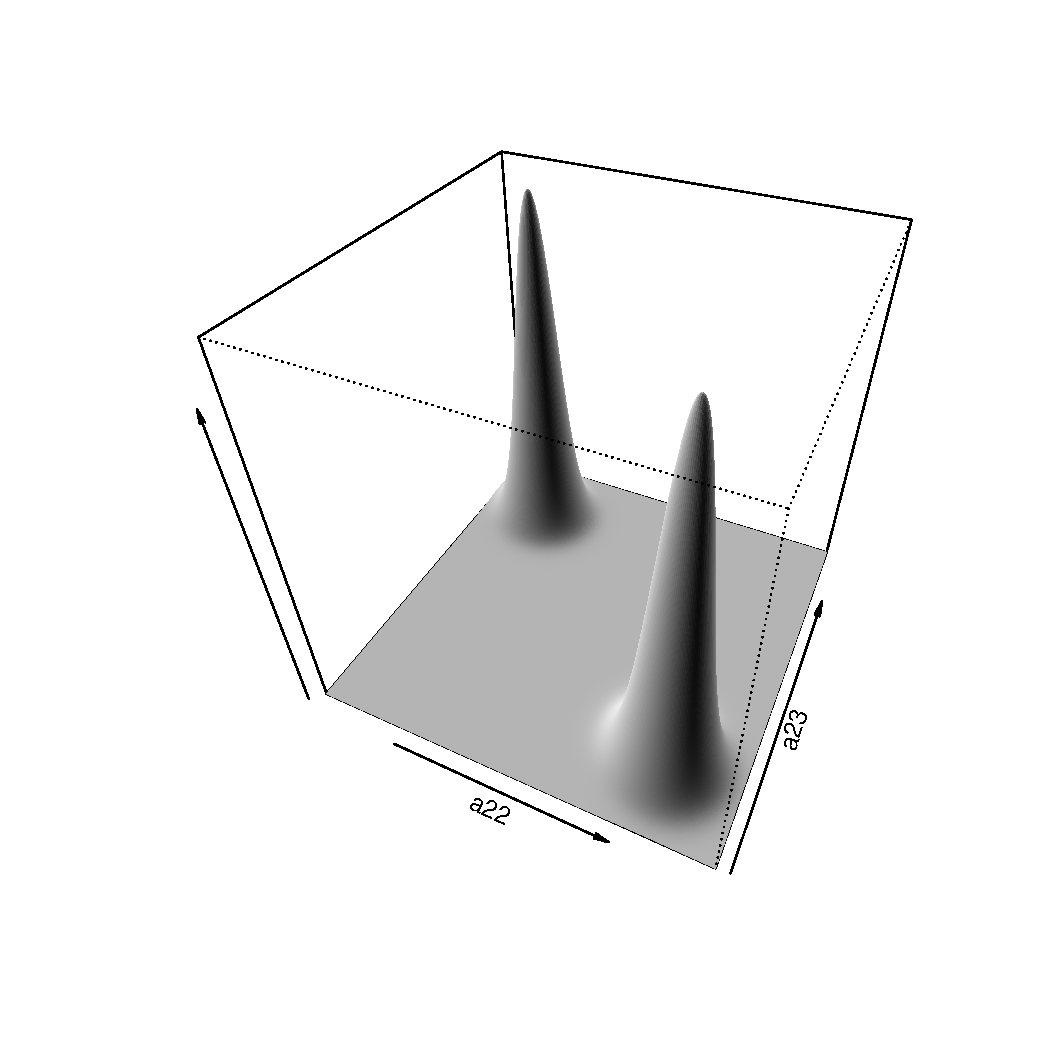
\includegraphics[scale=0.33, trim=2cm 1cm 2cm 1cm]{./Estimation/bi-density-22-23.pdf}&
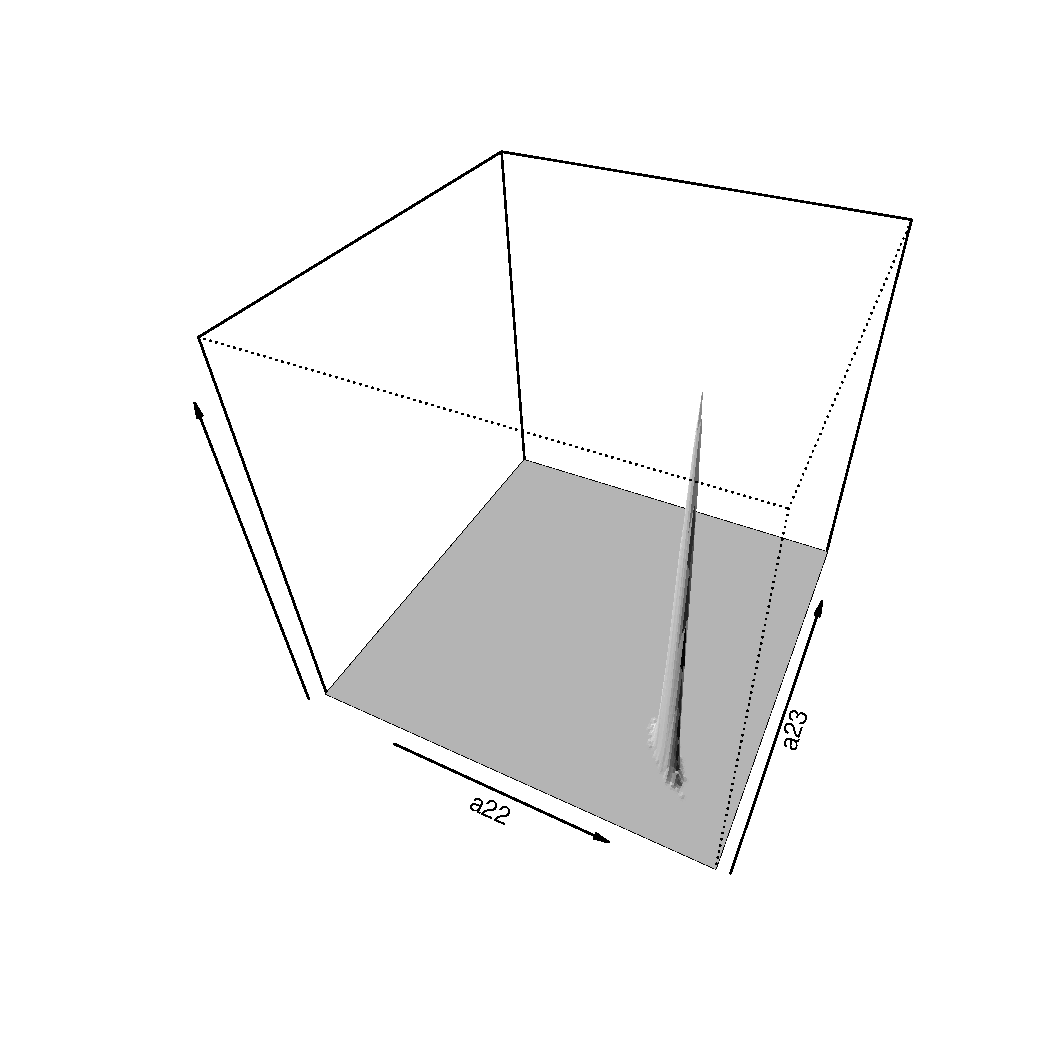
\includegraphics[scale=0.33, trim=2cm 1cm 2cm 1cm]{./Estimation/bi-density-22-23-n.pdf}\\
\multicolumn{2}{c}{bivariate densities: $(a_{22},a_{23})$}
\end{tabular}

\end{frame}






{\setbeamercolor{background canvas}{bg=mcxs2}
\begin{frame}{\color{mcxs1}Structural VARs: Gibbs sampling}

\textbf{The Gibbs sampler by Waggoner \& Zha (2003)}
\bigskip\begin{description}
\item[Thanks to] {\color{mcxs4}simple derivations an efficient sampler is feasible}

\smallskip\item[The sampler] {\color{mcxs4}draws the SF parameters directly}

\smallskip\item[Many extensions] {\color{mcxs4}in the specification of the model are possible}

\smallskip\item[Normalization] {\color{mcxs4}provides a solution to identification of the shocks up to their signs (a rotation matrix $D$)}
\end{description}
\end{frame}
}


\end{document} 